\section{ХОД РАБОТЫ}

\subsection{Формулировка задачи}

Написать функцию для моделирования состояний цепи Маркова.
Входными параметрами этой функции выбрать вектор состояний,
вектор начальных вероятностей, матрицу вероятностей перехода и
число шагов (тактов).

Использовать эту функцию для моделирования реализации состояний длительностью
50 -- 100 тактов.
Реализацию вывести в графическом окне в виде графика.

Начальное состояние моделируется с использованием вектора
вероятностей начального состояния $ A $, а последующие --- с использованием
соответствующих векторов-строк матрицы вероятностей перехода~$ P $.

Исходные данные:
\begin{equation*}
P = \begin{pmatrix}
      0{,}6 & 0 & 0{,}4 \\
      0{,}4 & 0{,}6 & 0 \\
      0{,}4 & 0{,}2 & 0{,}4 \\
    \end{pmatrix},
A = \begin{pmatrix}
      0{,}3 & 0{,}7 & 0
    \end{pmatrix},
E = \begin{pmatrix}
      5 & 6 & 7
    \end{pmatrix}.
\end{equation*}


\subsection{Теоретические сведения}

Определение. Цепью Маркова называется случайна последовательность
$\xi$, $ i = 0,1, ... $, если вероятность $ p_{i,j}^{s, s+1} $ того,
что в момент времени $ s+1 $ система будет находиться в состоянии $ E_j $,
зависит от того, в каком состоянии $ E_i $ система находилась в предыдущий момент
времени $ s $ и не зависит от того, в каких состояниях она находилась в более
ранние моменты времени $ s-1, s-2, ..., 0 $:
\begin{equation*}
  p_{i,j}^{s,s+1} = P(\xi_{s+1} = E_j / \xi_s = E_i) = P(\xi_{s+1} = E_j / \xi_s = E_i, \xi_{s-1} = E_k,...,\xi_0 = E_l).
\end{equation*}

Вероятность $ p_{i,j}^{s,s+1} = P(\xi_{s+1} = E_j / \xi_s = E_i) $ --- это условная
вероятность того, что в момент времени $ s+1 $ система будет находиться
в состоянии $ E_j $ при условии, что в предыдущий момент $ s $ она находилась
в состоянии $ E_i $. Это вероятность называется вероятностью перехода
из состояния $ E_i $ в состояние $ E_j $ за один шаг для моментов времени $ s, s+1 $.

Цепь Маркова называется конечной, если множество $ E $ ее состояний конечное.

Цепь Маркова называется однородной, если условная вероятность $ p_{i,j}^{s,s+1} $
не зависит от момента времени $s$. В этом случае такая вероятность обозначается
как $ p_{i,j} $ и называется вероятностью перехода из состояния $ E_i $ в состояние  за один шаг.

\pagebreak

\subsection{Ход работы}

Напишем функцию для моделирования состояний цепи Маркова. Входными параметрами
этой функции выберем вектор состояний, вектор начальных вероятностей,
матрицу вероятностей перехода и число шагов~(тактов). Используем эту
функцию для моделирования реализации состояний длительностью 30 тактов.
Полученные реализации изобразим в виде графика, который представлен
на рисунке~\ref{pic:chain}.
\begin{figure}[h]
  \centering
  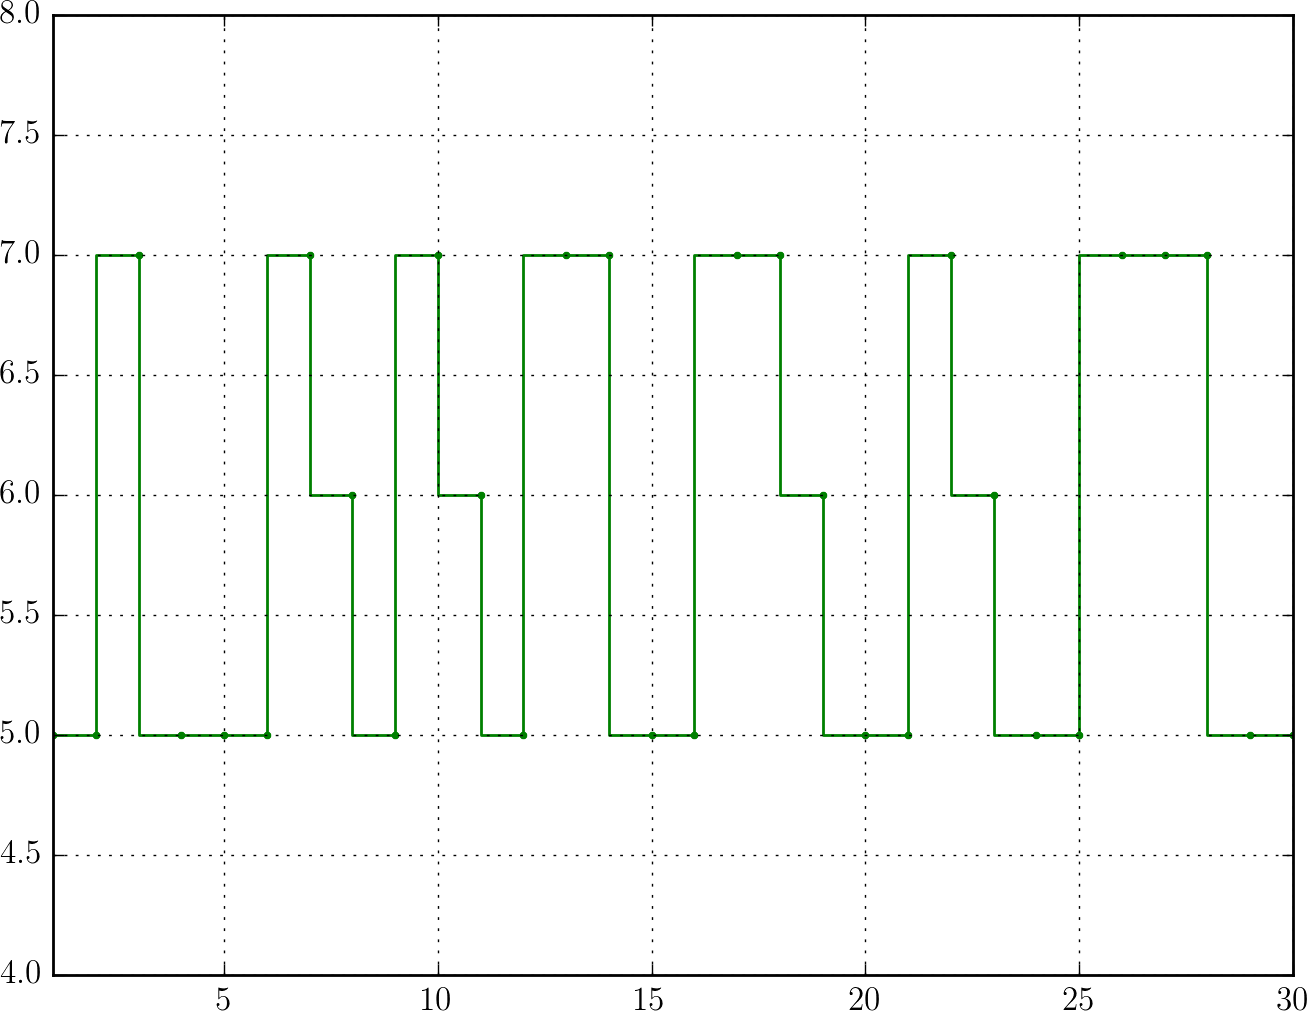
\includegraphics[width=150mm, height=92mm]{pic/chain}
  \caption{Последовательность случайных состояний,
    подчиненных Марковской зависимости}
  \label{pic:chain}
\end{figure}

Исходный код разработанной программы представлен в приложении~А.

\pagebreak